% Hybrid-pipeline schematic (vector redraw of method_overview.jpg).
% Wording matches the audited paper: the embedding module's drift signals fuse into
% the ChangeScore; the two modules combine in a fusion-and-ranking stage.
% Compile:  xelatex method_overview.tex
% Render :  pdftoppm -jpeg -r 600 -singlefile method_overview.pdf ../method_overview
\documentclass[border=6pt]{standalone}
\usepackage{helvet}\renewcommand{\familydefault}{\sfdefault}
\usepackage{tikz}
\usetikzlibrary{arrows.meta, positioning, fit, calc}
\begin{document}
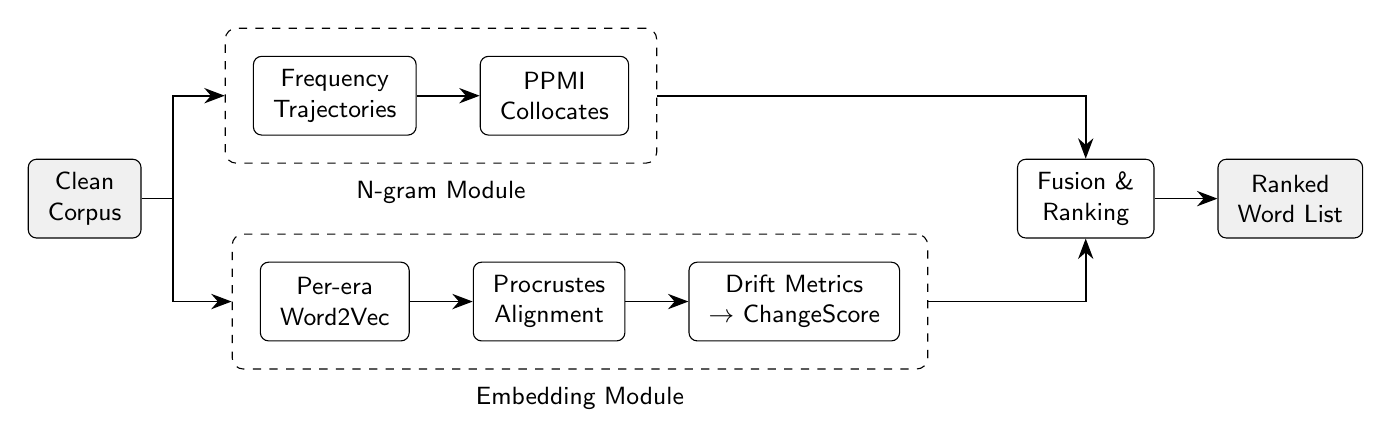
\begin{tikzpicture}[
  box/.style={draw, rounded corners=3pt, align=center, minimum height=10mm,
              inner xsep=2.5mm, font=\small},
  io/.style={box, fill=black!6},
  mod/.style={draw, dashed, rounded corners=4pt, inner sep=3.5mm},
  lab/.style={font=\small, anchor=north},
  arr/.style={-{Stealth[length=2.6mm]}, semithick}
]
  % n-gram module (top)
  \node[box] (freq) {Frequency\\Trajectories};
  \node[box, right=8mm of freq] (coll) {PPMI\\Collocates};
  % embedding module (bottom)
  \node[box, below=16mm of freq] (train) {Per-era\\Word2Vec};
  \node[box, right=8mm of train] (proc)  {Procrustes\\Alignment};
  \node[box, right=8mm of proc]  (drift) {Drift Metrics\\$\to$ ChangeScore};

  \node[mod, fit=(freq)(coll)]        (ngram) {};
  \node[lab] at (ngram.south)  [yshift=-1mm] {N-gram Module};
  \node[mod, fit=(train)(proc)(drift)] (embed) {};
  \node[lab] at (embed.south)  [yshift=-1mm] {Embedding Module};

  % input / fusion / output (fusion clears the wider embedding module's east edge)
  \node[io, left=11mm of $(ngram.west)!0.5!(embed.west)$]  (data) {Clean\\Corpus};
  \node[box] (fuse) at ($(embed.east |- data)+(20mm,0)$) {Fusion \&\\Ranking};
  \node[io, right=8mm of fuse] (out) {Ranked\\Word List};

  \draw[arr] (data.east) -| ++(4mm,0) |- (ngram.west);
  \draw[arr] (data.east) -| ++(4mm,0) |- (embed.west);
  \draw[arr] (freq)  -- (coll);
  \draw[arr] (train) -- (proc);
  \draw[arr] (proc)  -- (drift);
  \draw[arr] (ngram.east) -| (fuse.north);
  \draw[arr] (embed.east) -| (fuse.south);
  \draw[arr] (fuse) -- (out);
\end{tikzpicture}
\end{document}
